%%%%%%%%%%%%%%%%%%%%%%%%%%
%%%%%Related work
%%%%%%%%%%%%%%%%%%%%%%%%%%
\begin{comment}
\begin{table*}[ht]\label{compare} 

\small 

\begin{tabular} {|l |c | c| c| c| c| c| c| }

\hline

                            			     &Scalable Fine-         & Supersession     & No Routing    	 &   Interdomain    &    Middlebox        &  Endpoint  &  No Application\\
						     &Grained Control        & Liveness     	& Modification  	 &   Middlebox       &Migration       &  Mobility  & change \\\hline
SIMPLE,FlowTags~\cite{SIMPLE,FLOWTAGS}        	   & $\oslash$             & $\oslash$   	& $\otimes$     	 &   $\oslash$      &    $\oslash$       &  $\otimes$   \\ \hline
OpenNF,Split/Merge~\cite{OpenNF,splitmerge}         & $\otimes$             & $\odot$     	& $\otimes$     	 &   $\oslash$      &    $\odot$         &  $\otimes$  \\ \hline
CoMB~\cite{CoMB}             & $\odot$               & $\odot$     	& $\odot$       	 &   $\otimes$        &    $\otimes$       &  $\otimes$ \\ \hline 
DoA~\cite{DOA}               & $\otimes$             & $\odot$    	 & $\odot$     	 	  &   $\odot$        &    $\otimes$       &  $\otimes$  \\ \hline
APLOMB~\cite{Aplomb}         & $\otimes$             & $\otimes$  	 & $\otimes$  	   	 &   $\odot$        &    $\odot$         &  $\otimes$ \\ \hline
Software Routing~\cite{OVS, click} & $\odot$         & $\otimes$  	 & $\odot$      	  &   $\odot$        &    $\oslash$       &  $\otimes$  \\ \hline



\end{tabular}
\caption{\small Comparison between different middlebox traffic steering solutions and mobility protocols ($\odot$ indicates that a scheme fully supports the criterion; $\otimes$ indicates a scheme does not, $\oslash$ indicates partially support or can be extended to) }
\end{table*}
\end{comment}




\section{Motivating Examples}

In this section, we first present a few scenarios where a system may require network function (NF) insertion, removal, or migration, and host mobility. We also discuss how the current solutions fail to address our requirements.


\subsection{Dynamic NF Policy}
Enterprise networks deploy various network functions for better performance and security. Being able to modify dynamically NF types/instances in a service chain improves the efficiency and flexibility of the network system. NF insertion is necessary if a flow is marked as suspicious by a coarse-grained intrusion detection and prevention system (IDPSs~\cite{IPS}) and requires a fine-grained deep packet inspection (DPI). NF removal is preferred if a connection goes through a cache proxy, but the proxy has a cache-miss and the content is uncacheable; the cache proxy may remove itself from the chain. NF load balancing is necessary if the network operators want to distribute a flow evenly among multiple instances of the same NF. Moreover, NF instance migration can happen in a network function virtualization (NFV) setting, and the flows that use the NF instance also need to migrate along with the instance. 

% \subsection{Case Study}
\begin{figure}[ht]
\centering
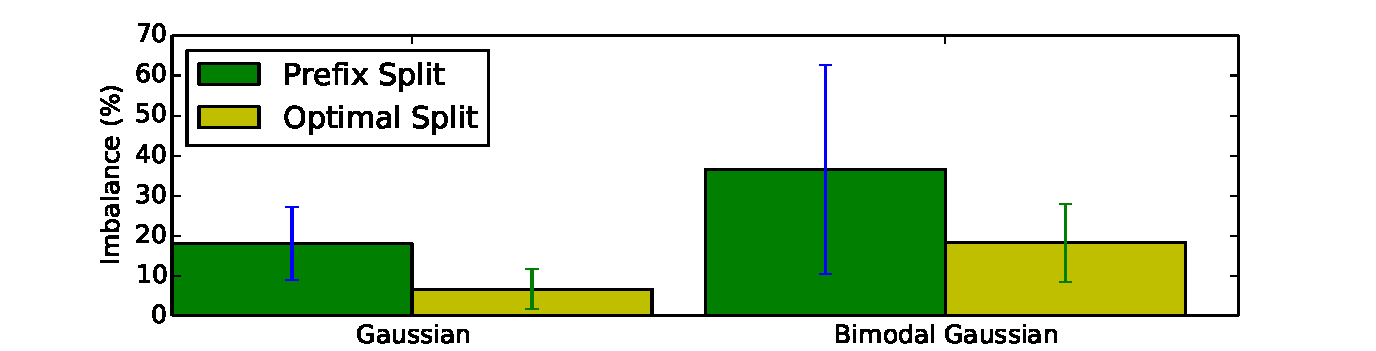
\includegraphics[width=\linewidth]{figures/routingsucks.pdf} 
\caption{\small The distribution of flow size for different prefix can be
measured using a weight\protect\cite{Niagara}. We assume two different weight
distributions for IP prefix: Gaussian, Bimodal  Gaussian with the parameters from\protect\cite{Niagara}. 
We show that in the  case of distributing flow over two  NF instances, a
routing solution, while doubling rules, fails to balance the load across middleboxes in the scenario
above. (Prefix split uses the most significant bit, and optimal split uses arbitrary one bit wildcard matching).} \label{distribution}
\end{figure}
% 


Efficient, dynamic NF policies cannot be implemented on conventional switches due to coarse-grained routing, e.g., the switch may simply tunnel all the traffic to IDS for further inspection and remove the IDS once it finds the proverbial ``needle in the haystack''. Some recent techniques leverage fine-grained routing switches (e.g., OpenFlow~\cite{openflow} based) for dynamically changing NF policies. However, these solutions are neither scalable due to TCAM rule size, nor flexible due to a complex dependency between routing rules. The SDN controller plays an excessive role in data plane, while still fails to fulfill certain network order-preserving properties~\cite{splitmerge, OpenNF}. Figure~\ref{distribution} gives an example of the imbalance caused by routing solution when trying to distribute flows across two instances of the same NF type. 

\subsection{Mobility and NF Policy} 
A cellular network can be divided into user equipment (UE), local access network (LAN) and core network.  LANs communicate to UEs through its base station and communicate to the Internet through the core network. Cellular networks rely on a wide range of NFs (e.g., firewall~\cite{IPTABLES}, load balancer~\cite{balance}, cache proxy~\cite{squid}) to improve performance and enhance security. As mobility and network function virtualization become ubiquitous, we may ask for (i) seamless mobility and (ii) dynamic service chaining.

Many mobility solutions have been proposed over the past years~\cite{mip, TCPMobile, I3Mobile, serval}, yet none of them consider the existence of network functions. Worse, NFs can even be a hindrance for these protocols since they may interfere with the protocol control logic (e.g., TCP split~\cite{TCPProxy}). Routing-based solutions have been proposed for service chaining in cellular networks(e.g., SoftCell~\cite{softcell}). However, in order to support host mobility, it places NFs only in the core network and does not support dynamic service chaining. 


